\documentclass[12pt, a4paper]{ntut-report}
\usepackage[dvips,xetex]{graphicx}
\usepackage{ifpdf,mla}% <-- mla.sty requires ifpdf.sty, but (perversely) doesn't load it
\usepackage{fontspec}
\usepackage{geometry}
\usepackage{lipsum}
\usepackage{xeCJK}
\usepackage{wallpaper}
\usepackage{pdfpages}
\usepackage{indentfirst}
\usepackage{setspace}
\usepackage{hyperref}
\usepackage{zhnumber}
\usepackage{titlesec}
\usepackage{amsmath}
\usepackage[backend=bibtex,sorting=none,style=ieee]{biblatex}   
\usepackage{algorithm}
\usepackage{algpseudocode}
\usepackage{float}
%\usepackage[linesnumbered,ruled,vlined]{algorithm2e}


\renewcommand{\baselinestretch}{1.5}
\xeCJKsetup{AutoFakeBold=true, AutoFakeSlant=true}
\setCJKmainfont{標楷體} % 中文字體
\setmainfont{Times New Roman} % 英文字體
\geometry{a4paper,total={297mm,210mm},top=4.5cm,bottom=0.75cm,left=2.5cm,right=2.5cm} % 頁面設定,不需修改
\pagestyle{plain} % 頁碼
\addbibresource{reference.bib}

%
% this file is encoded in utf-8
%

%% 這些設定值將會用於呈現在首頁上,請進行填入
%% Please fill in the information which will be shown on the cover and in the abstract. All Chinese and English information must be matched to each other. If you don’t have any Chinese information, please skip the Chinese ones, but all English Information is required.

%
% 中文論文設定值,請根據以下的範例進行填入
%

% 論文題目(中文)
% Thesis Title (Chinese)
\newcommand\cTitle{基於沙盒系統之程式評測應用}

% 我的姓名(中文)
% My Name(Chinese)
\newcommand\myCname{黃漢軒}

% 指導教授的姓名 (中文),使用頓號隔開 
% Advisor (Chinese), use “、” to separate names
\newcommand\advisorCname{郭忠義 博士}

% 校名 (中文)
% School Name(Chinese)
\newcommand\univCname{國立臺北科技大學}

% 系所名 (中文)
% Department Name(Chinese)
\newcommand\deptCname{資訊工程系碩士班}

% 學位名 (中文)
% Degree Name(Chinese)
\newcommand\degreeCname{碩士}

% 口試年份 (中文、民國)
% Year of Oral Defense(Chinese)
\newcommand\cYear{一百一十二}

% 口試月份 (中文)
% Month of Oral Defense(Chinese)
\newcommand\cMonth{七} 

% 畢業學年度 (中文)
% 如 112 學年度第2學期畢業,當時為民國113年6月,學年度即為112,不是113。
\newcommand\cAcademicYear{一百一十二}

% 畢業學期(中文)
% Academic Year (Chinese)
\newcommand\cGraduateSemester{二}

%
% 英文論文設定值,請根據以下的範例進行填入
%

% 論文題目 (英文)
% Thesis Title (Engslih)
\newcommand\eTitle{Online Judge System based on Sandbox System}

% 我的姓名(英文)
% My Name(English)
\newcommand\myEname{Huang, Han-Xuan}

% 指導教授的姓名 (英文),使用逗號隔開
% 例如:Dr. Kuo Jong-Yi, Dr. A B-C, ...
%
% Advisor (Ensligh), use “, ” to separate names
% e.g. Dr. Kuo Jong-Yi, Dr. A B-C, ...
\newcommand\advisorEname{Dr. Kuo Jong-Yi}

% 校名(英文)
% School Name(English)
\newcommand\univEname{National Taipei University of Technology}

% 系所全名 (英文)
% Department Name(English)
\newcommand\fulldeptEname{Department of Computer Science and Information Engineering}

\newcommand\deptEname{Computer Science and Information Engineering}

% 學位名 (英文)
% Degree(English)
\newcommand\degreeEname{Master of Science}

% 口試年份 (阿拉伯數字、西元)
% Year of Oral Defense(English)
\newcommand\eYear{2023}

% 口試月份 (英文)
% Month of Oral Defense(English)
\newcommand\eMonth{June}

%畢業級別;用於書背列印;若無此需要可忽略
\newcommand\GraduationClass{111}

%%%%%%%%%%%%%%%%%%%%%%

\begin{document}

% 封面、不用浮水印 Cover without a watermark
%\begin{titlepage}
    \newpage
    \begin{center}
        % 北科的 Logo
        
\includegraphics[width=13cm]{ntut-logo-with-label.png}
        
        % 北科的系所名與學位名,以換行隔開
        \huge\bf\deptCname\\% 系所名
        \huge\bf\degreeCname 學位論文\\% 學位名
        % \huge\bf\fulldeptEname \\% 系所英文名
        % \huge\bf\degreeEname Thesis \\ % “Master Thesis” or “Ph.D. Dissertation”

        % 中文與英文論文名稱
        % 如果你不需要英文,你可以註解 \eTitle
        \vfill
        \huge\bf\cTitle\\ %%%%%
        \LARGE\bf\eTitle\\ %%%%%

        % 研究生(中文)
        \vfill
        {\Large 研究生:\myCname}
        %  {\Large Researcher: \myEname}

        % 指導老師(中文)
        \vfill
        {\Large 指導教授:\advisorCname}
        % {\Large Advisor: \advisorEname}

        % 畢業年份(中文)
        \vfill
        {\Large 中華民國{\cYear 年}{\cMonth 月}}
        %  {\Large \eMonth, \eYear}
    \end{center}
\end{titlepage}
% 留白頁、不用浮水印 Blank page without a watermark
\newpage
\thispagestyle{empty}
\null
\newpage
% (預留空白頁)

% 新增浮水印 Add Watermarks
\CenterWallPaper{.64}{ntut-logo.png}

% 封面、要浮水印 Cover with a watermark
\begin{titlepage}
    \newpage
    \begin{center}
        % 北科的 Logo
        
\includegraphics[width=13cm]{ntut-logo-with-label.png}
        
        % 北科的系所名與學位名,以換行隔開
        \huge\bf\deptCname\\% 系所名
        \huge\bf\degreeCname 學位論文\\% 學位名
        % \huge\bf\fulldeptEname \\% 系所英文名
        % \huge\bf\degreeEname Thesis \\ % “Master Thesis” or “Ph.D. Dissertation”

        % 中文與英文論文名稱
        % 如果你不需要英文,你可以註解 \eTitle
        \vfill
        \huge\bf\cTitle\\ %%%%%
        \LARGE\bf\eTitle\\ %%%%%

        % 研究生(中文)
        \vfill
        {\Large 研究生:\myCname}
        %  {\Large Researcher: \myEname}

        % 指導老師(中文)
        \vfill
        {\Large 指導教授:\advisorCname}
        % {\Large Advisor: \advisorEname}

        % 畢業年份(中文)
        \vfill
        {\Large 中華民國{\cYear 年}{\cMonth 月}}
        %  {\Large \eMonth, \eYear}
    \end{center}
\end{titlepage}
% 「學位論文口試委員會審定書」掃描檔,請檢附完整簽名之審定書掃描檔
% Please add "Oral Defense Committee Signature Form" with complete signatures.
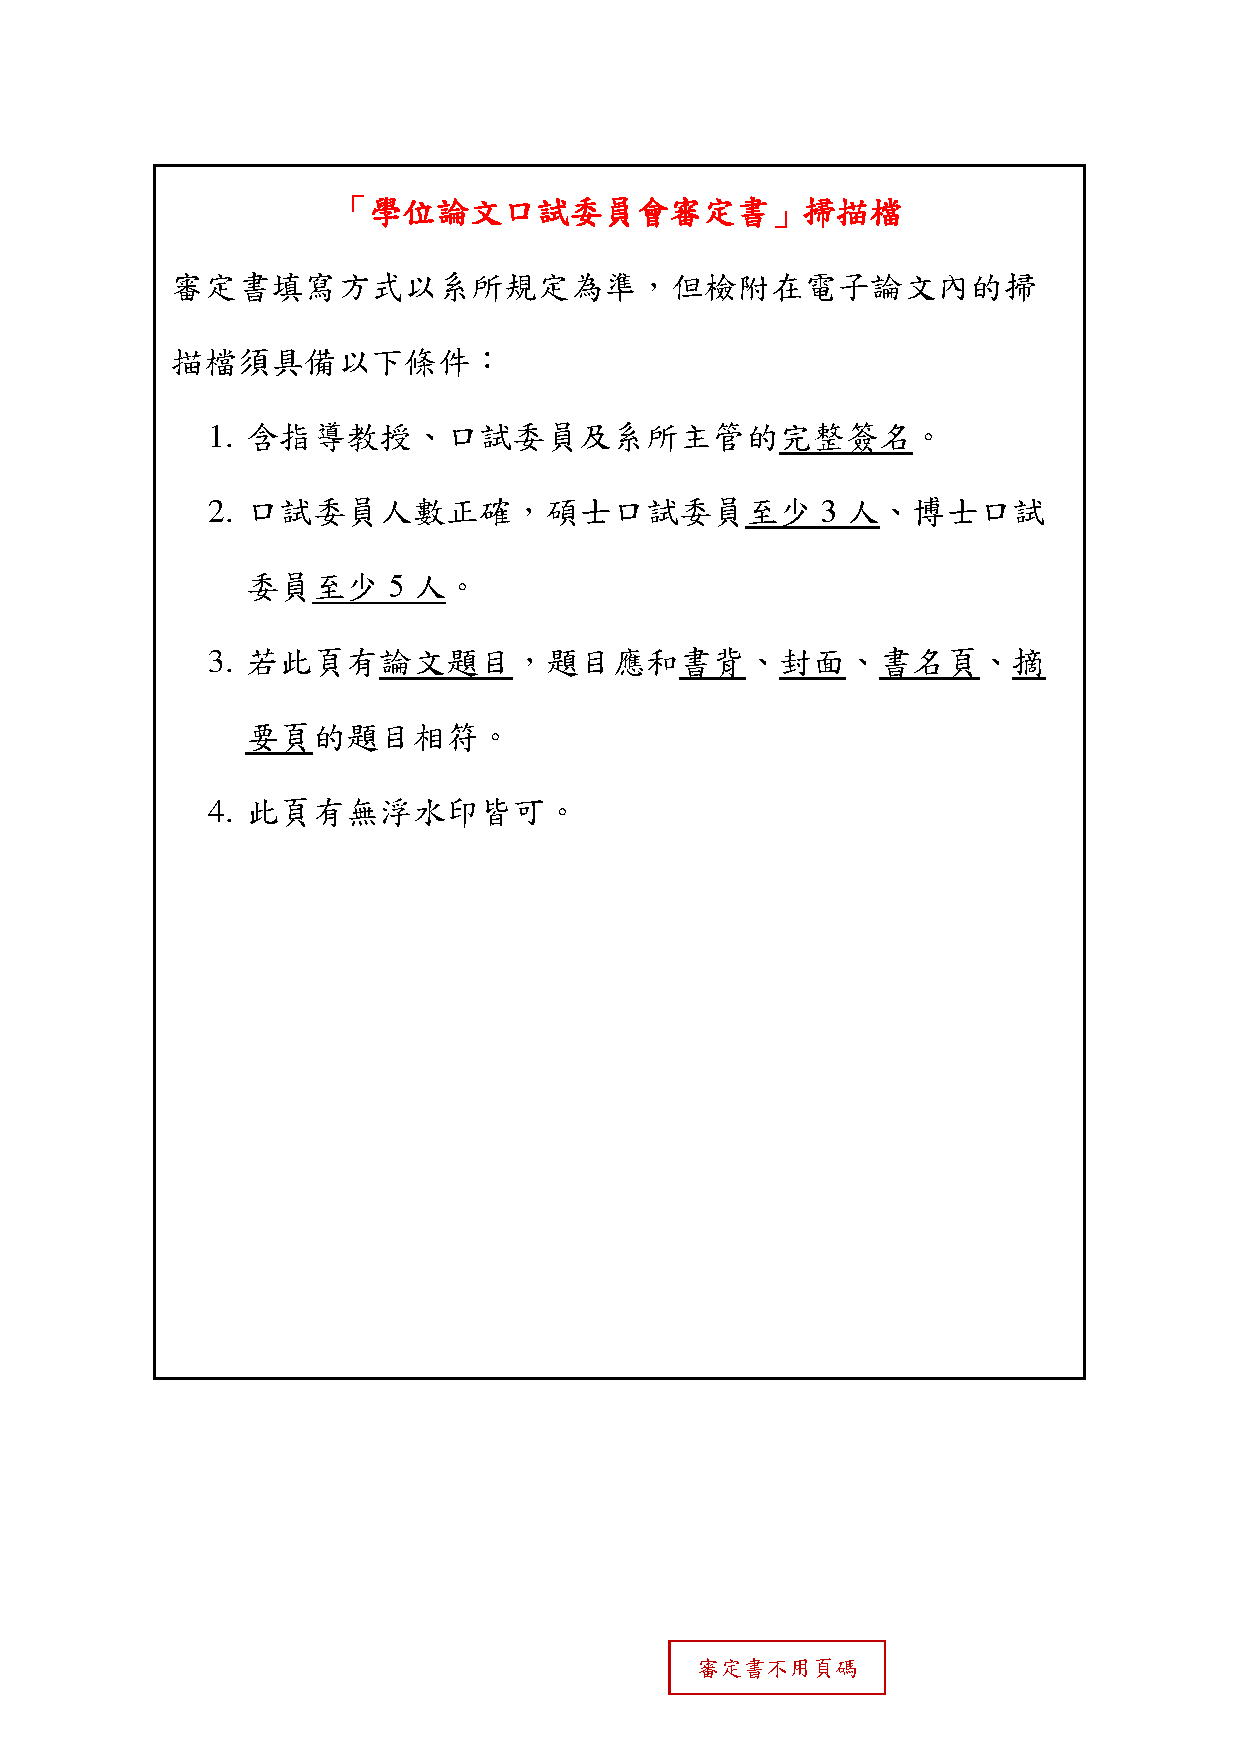
\includepdf[pages=-,offset=0cm -2.5cm]{static-page/signpage.pdf}

\pagenumbering{roman}

% 摘要頁(中文)Abstract (Chinese)
% If you don’t have Chinese abstract, please delete this one.
% 中文摘要頁
\begin{ZhAbstract}
    \begin{ZhAbstractItems}
        % 關鍵詞,請自己填,請自己填,多個關鍵字以逗號(、)隔開
        \noindent \text 關鍵詞:(請自己填)

    \end{ZhAbstractItems}

    \begin{ZhAbstractDescription}
        摘要為論文或報告的精簡概要,其目的是透過簡短的敘述使讀者大致瞭解整篇報告的內容。摘要的內容通常須包括問題的描述以及所得到的結果,但以不超過 500 字或一頁為原則,且不得有參考文獻或引用圖表等。以中文撰寫之論文除中文摘要外,得於中文摘要後另附英文摘要。標題使用 20pt 粗標楷體並於上、下方各空一行(1.5 倍行高,字型 12pt 空行)後鍵入摘要內容。摘要頁須編頁碼(小寫羅馬數字表示頁碼)。
    \end{ZhAbstractDescription}
    
\end{ZhAbstract}


% 摘要頁(英文)Abstract (English)
% 英文摘要頁
\begin{EnAbstract}
    \begin{EnAbstractItems}
        % 關鍵詞,請自己填,多個關鍵字以逗號 "," 隔開
        \noindent \text Keyword: (Fill it)

    \end{EnAbstractItems}

    \begin{EnAbstractDescription}
        Start writing abstract from here. Start writing abstract from here. Start writing abstract from here. Start writing abstract from here. Start writing abstract from here. Start writing abstract from here. Start writing abstract from here. Start writing abstract from here.
    \end{EnAbstractDescription}
    
\end{EnAbstract}


% 鳴謝 Acknowledgements
\begin{Thanks}
    所有對於研究提供協助之人或機構,作者都可在誌謝中表達感謝之意。
\end{Thanks}
% 目錄、表目錄與圖目錄 Table of Contents, List of tables, List of figures
\begin{TableOfContent}
    \tableofcontents
\end{TableOfContent}

\begin{TableOfContent}
    \listoffigures
\end{TableOfContent}

\begin{TableOfContent}
    \listoftables
\end{TableOfContent}
 
\pagenumbering{arabic}

% 章節一 Chapter 1
\begin{ZhChapter}

\chapter{緒論}

\section{研究背景}

科技的快速進步,讓人們的生活更加便利,物聯網(IoT)的應用已經與日常生活密不可分,包含了醫療及工業的應用,無所不在,\cite{mordor2024iot}根據日商環球訊息有限公司(GII)調查,物聯網(IoT)市場規模預計從2024年到2029年,將從1.17兆美元增加至2.37兆美元,年均複合成長率(CAGR)為15.12\%,如圖\ref{fig: IoT市場規模評估}所示。

\begin{figure}[H]
    \centering
    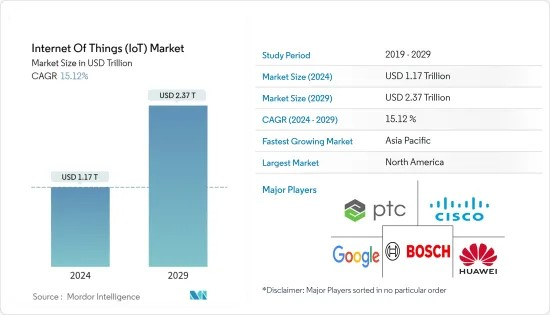
\includegraphics[width = 1\textwidth]{image/market_research.jpg}
    \caption{IoT市場規模評估\cite{mordor2024iot}}
    \label{fig: IoT市場規模評估}
\end{figure}

2010年6月藍牙技術聯盟(Bluetooth Special Interest Group)提出了低功耗藍牙(Bluetooth Low Energy, BLE),BLE省電及低成本的特性,使得藍牙技術在物聯網(IoT)的應用種佔據了不可或缺的角色,例如:目前市面上的無線設備包括藍牙耳機、藍牙鍵盤及藍牙滑鼠。
物聯網(IoT)的應用中,大量使用無線感測網路(Wireless Sensor Networks, WSN),會在環境之中分布許多的節點,而節點不只有當作感知器測量環境的數據,常常還要當作中繼節點,轉傳發送端與目的端的封包,最終將所有量測的數據匯集到終端節點,以監控所有的節點數據,將數據儲存後,進行分析後並做出適當的處理,也可以透過分析數據預測環境的變化,並提前做出適當的處理。

藍牙網狀網路(Bluetooth Mesh)架構的實現,讓BLE更具有可靠性(Reliability)及擴展性(Scalability),可以允許多個BLE裝置相互連接並形成網狀結構,讓封包可以在多個裝置之間進行傳輸,讓傳輸距離不會受到單一裝置的傳輸範圍限制,解決了節點之間裝置連接數量的限制以及傳輸距離不足的問題,在物聯網(IoT)的應用,例如:智慧建築、智慧工業、智慧城市、智慧家庭..等等,BLE都已經扮演重要也不可或缺的角色。
	
%在物聯網(IoT)與藍牙網狀網路(Bluetooth Mesh)中,對整個系統架構做出適當的評估,在不影響裝置效能的情況下,設計多個藍牙裝置之間的分流機制,因為在整個系統中,流量可能會有所起伏,為了讓每個裝置可以有一樣的傳輸品質,且系統可以發揮最好的吞吐量。
	

\section{研究動機與目的}

FruityMesh是一個專門為BLE Mesh Network所開發的開源網路協定框架。在文獻\cite{112TIT00392032}中的研究,發現在原生FruityMesh上封包傳輸是採用廣播的方式,向相鄰的所有節點發送封包,這種設計雖然簡單,卻容易導致大量冗餘封包的產生,這會導致節點之間傳輸不必要的封包,最終導致整個BLE Mesh出現廣播風暴。因此\cite{112TIT00392032}作者針對FruityMesh傳輸時產生的廣播風暴,提出了DOT(Destination Oriented Transmission)排程的機制,將BLE Mesh導入樹狀傳輸結構,對整個系統進行分層管理,讓封包傳輸只會向目的端正確的路徑上傳輸,避免了廣播風暴的產生。作者在研究過程中,也發現BLE Multi-Hop網狀網路節點會擁有Master以及Slave兩種角色,而在同一個時間下,節點同時會是Master和Slave的狀態,而這種狀態上的衝突會導致的封包傳輸產生遺失現象。

\cite{112TIT00392032}作者為了解決角色衝突的問題,在DOT的架構下增加啟用以及禁用的機制,提出DOST(Destination Oriented Switch Transmission)的排程設計,利用時間交錯方式讓裝置在同一個時間只會扮演Master或Slave,解決在同一個時間點節點可能會因為扮演Master及Slave角色衝突而導致的封包傳輸遺失的問題;因此,在FruityMesh中導入DOST設計後已經改善了大部分的封包傳輸延遲以及封包重傳率,但仍存在些許效能瓶頸,因為在無線網路中,所有節點的封包傳輸都是透過無線電波,以廣播的方式傳輸,這會導致在多個節點同時傳輸封包時,可能會產生封包碰撞的問題,導致封包傳輸延遲增加。


此外,\cite{112TIT00392032}文獻指出,若要在 DOST 架構下進一步提升效能,需確保拓樸建立時,Sink 節點為整體網路的根節點。然而原研究並未針對拓樸控制機制提出具體解法。若未能確保 Sink 位於樹根,當其斷線並重新加入網路時,可能無法恢復為原先的根節點角色,進而影響整體傳輸路徑的穩定性與效能。

在\cite{112TIT00392032}\cite{110TIT00392037}中,針對了single hop 及 multi hop mesh的網路拓樸進行探討,當使用合適的封包連接參數可以有效降低封包傳輸延遲及重傳率;\cite{109TIT00392031}中,探討了 single hop 星狀網路下在不同封包大小的情形下,計算出最適合的連接參數,在傳輸過程動態調整連接的CE(Connection Event)及CI(Connection Interval),達到更好的吞吐量。

%本計畫將研究中在DOT的排程設計下,仍然會有些許因為封包遺失,而產生的封包重傳的問題,以及在藍牙網狀網路(Bluetooth Mesh)架構,執行TDMA的排程機制,結合調整連線參數,確保傳輸品質,並修改FruityMesh拓樸方法,讓BLE Mesh建立的過程確保Sink點在整個樹狀結構的根節點,也確保Sink點如果斷線後重新連線後依然是整個BLE Mesh樹狀結構的根節點。

本計畫針對現有 DOT 架構下,進一步改善 FruityMesh 的拓樸建立方法,使藍牙網狀網路在建立初期便能確保 Sink 節點為整個樹狀結構的根節點,並透過調整節點連線策略與連接排序邏輯,讓 Sink 節點即使在斷線後重新加入網路,也能恢復為原先的根節點角色,維持拓譜的穩定。

此外現有 DOT 架構下仍可能發生的封包遺失與重傳現象,為進一步改善高負載環境下的傳輸品質,本研究設計一套階層式的 Connection Interval(CI)調整機制。根據節點在網路拓樸中的階層位置進行分級設定,因越接近 Sink 的節點承擔更多封包轉發與回應任務,故分配較短的 CI,第一層為 25ms,第二層為 50ms,第三層為100ms,讓越接近 Sink 的節點增加可用的傳輸時段,降低擁塞與傳輸延遲。此機制不僅可有效緩解 Sent Buffer 的壓力,亦可提升整體封包遞送成功率(Packet Delivery Ratio)、降低封包重傳率(Packet Retransmission Rate)與平均封包延遲(Average Packet Delay),進而強化整體 Mesh 網路的穩定性與效能。

\section{論文架構}
本論文共分為五章,第一章說明本研究的背景與動機,並闡述本論文所要解決的問題與研究目的。

第二章整理並探討本研究所依據的基礎知識與技術背景,包括藍牙低功耗(BLE)通訊技術、藍牙網狀網路(BLE Mesh)架構、BLE 中的排程與連線機制(如 CI、CE)、以及目的地傾向傳輸策略。此外,也介紹本研究所採用的開發平台,包含 Nordic Semiconductor 所推出的 nRF52840 晶片與 SoftDevice 堆疊,以及基於該硬體的 FruityMesh 開源框架,並進一步說明 FruityMesh 的 Cluster 與 Self-Healing 機制。

第三章分析現有 FruityMesh 在拓樸建立與封包傳輸上可能出現的問題。接著提出改良的拓樸建立演算法與設計,包括以 Master 或 Slave 身分進行最佳連線選擇,以及改善自我修復(Self-Healing)行為的拓樸重建機制。此外,本章亦設計改善封包傳輸效能的對應策略,以確保在多節點環境下依然能維持高效通訊。

第四章說明本研究之實驗設計與評估方式,分別建置實體測試平台與模擬平台(CheerySim)以模擬不同節點規模下的網路拓樸生成與封包傳輸行為。實驗部分以多組節點數模擬進行測試,並設計多項效能評估指標,包括拓樸建立時間、自我修復時間、平均 HopsToSink 數值、封包傳輸延遲、封包抵達率與封包重傳率,藉此全面評估所提出機制的實際效能表現。

第五章總結本研究的成果與貢獻,並探討未來在 BLE Mesh 網路設計中可延伸的研究方向與改進空間,期望能為低功耗網狀通訊領域提供可參考之實作架構與演算法設計依據。


\end{ZhChapter}
% 章節二 Chapter 2
\begin{ZhChapter}

\chapter{相關技術與背景}

\section{藍牙低功耗技術}

藍牙技術聯盟(Bluetooth Special Interest Group)在2010年6月發布了可以短距離數據交換和低功耗的藍牙低功耗技術(Bluetooth Low Energy, BLE)。而藍牙低功耗技術被發布後,就被物聯網(IoT)廣泛的應用,包括了家庭娛樂、醫療保健、運動健身、安防以及信標等領域。

藍牙低功耗技術(Bluetooth Low Energy, BLE)是一種功耗極低的技術,這一個技術讓裝置在大部分的時間都在休眠模式,只有在需要使用該裝置時,才會快速喚醒進行工作,這讓BLE裝置僅需要一顆鈕扣電池就可以運作數月甚至數年之久,這讓BLE生產成本更低,且保留了傳統藍牙(Classic Bluetooth)類似的通訊範圍,且一樣相容於手機、平板電腦等設備。

BLE運作在2.4G的ISM頻段,利用FDMA(Frequency Division Multiple Access),將2402MHz至2480MHz分成40個Channel,又將這些Channel又分成兩種傳輸模式,廣播模式(Advertising Mode)及連線模式(Connection-Oriented Mode),其中廣播模式使用了Channel 37、Channel 38、Channel 39,工作頻率分別是2403MHz、2426MHz、2480MHz,剩餘的37個Channel為連接模式使用,如圖\ref{fig: 廣播頻道與資料頻道示意圖}所示。

\begin{figure}[H]
    \centering
    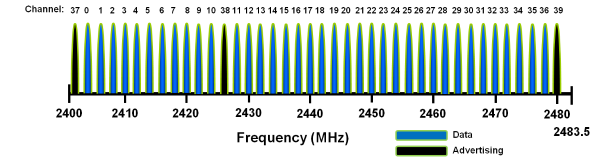
\includegraphics[width = 1\textwidth]{image/ble-phy-channel-assignment.png}
    \caption{廣播頻道與資料頻道示意圖\cite{microchip2023}}
    \label{fig: 廣播頻道與資料頻道示意圖}
\end{figure}

廣播模式和連接模式的運作機制由 BLE 的控制層(Controller Layer)狀態機管理,包括Standby(等待)、Advertising(廣播)、Scanning(掃描)、Initiating(初始化)、Connection(連接)五種狀態 ,如圖\ref{fig: Controller layer 狀態機示意圖}所示。

\begin{figure}[H]
    \centering
    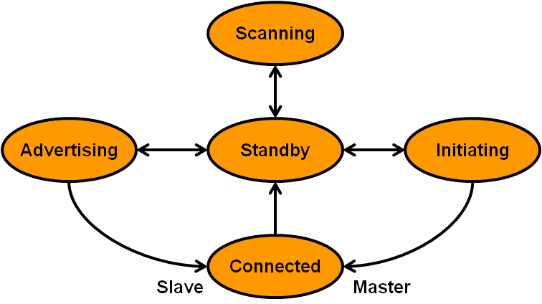
\includegraphics[width = 1\textwidth]{image/ble-link-layer-sm.png}
    \caption{Controller layer 狀態機示意圖\cite{microchip2023}}
    \label{fig: Controller layer 狀態機示意圖}
\end{figure}

\subsection{廣播模式}

在廣播模式 (Advertising Mode)中,會使用Channel 37、Channel 38、channel 39這三個廣播頻道,主要用於掃描裝置、建立通訊頻道和廣播的傳輸,其中廣播者(Advertiser)是由待機狀態(Standby Status)進入廣播狀態(Advertising Status),廣播者會在三個廣播頻道輪流發送廣播封包,讓掃描者(Scanner)可以檢測到其存在,並提供基本的數據,例如:裝置名稱或狀態。

掃描者(Scanner)是由待機狀態(Standby Status)進入掃描狀態(Scanner Status),掃描者會輪流掃描三個廣播頻道的廣播封包,以接收範圍內的所有廣播的資訊,掃描收集數據後,準備與廣播設備建立連接,如圖\ref{fig: 廣播模式示意圖}所示。
\begin{figure}[H]
    \centering
    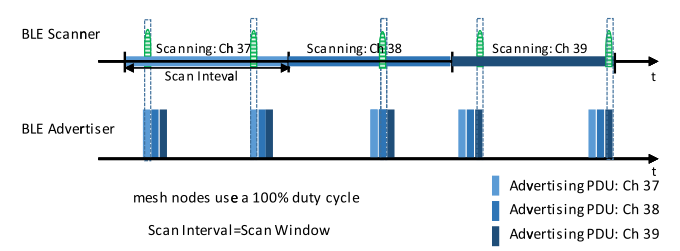
\includegraphics[width = 0.8\textwidth]{image/廣播模式示意圖.png}
    \caption{廣播模式示意圖\cite{9035389}}
    \label{fig: 廣播模式示意圖}
\end{figure}

\subsection{連接模式}

連接模式(Connection-Oriented Mode)中,設備需要首先透過廣播模式建立連接,其中廣播者(Slave)負責發送連線請求的廣播封包,而掃描者(Master)檢測到廣播封包後,從 Standby 進入 Scanning,再進入 Initiating 狀態,開始與廣播設備握手 (Handshake)。

當握手成功後,雙方進入 Connection 狀態。連接建立後,Master 與 Slave 可通過剩餘的 37 個數據頻道進行數據傳輸;Master 負責與多個 Slave 的連線管理,分配專屬的時間槽 (Time Slot) 給各連接設備,即使沒有數據需要傳輸,系統仍會保留固定的時間槽以確保系統的穩定性,避免通訊衝突。圖\ref{fig: 連線模式示意圖}為連線模式示意圖。

\begin{figure}[H]
    \centering
    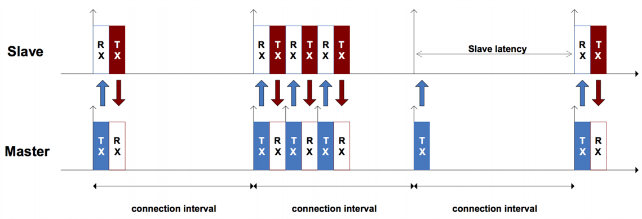
\includegraphics[width = 0.9\textwidth]{image/連線模式示意圖.png}
    \caption{連線模式示意圖\cite{9035389}}
    \label{fig: 連線模式示意圖}
\end{figure}

\subsection{BLE排程機制}

廣播者(Advertiser)和掃描者(Scanner)會在建立連線後,進行數據的交換,當掃描者在三個掃描頻道掃瞄並偵測到廣播者發送的封包後,掃描者會在約 150 微秒($T_{IFS}$)後回應一個 CONNECT\_IND 封包。CONNECT\_IND 封包包含了多項管理連接的參數,例如:影響錨點時間(Anchor Point, AP)的 WinSize 以及 WinOffset。

這些連接參數,Connection Interval (CI)、Anchor Point (AP)和Connection Event (CE)對於裝置之間的排程機制影響非常大,在一個Connection Interval(CI)的時間內,一個Slave裝置只會與Master裝置有一個Connection Event(CE)傳輸時間來進行資料的交換,所以Connection Interval(CI)的時間影響Connection Event(CE)的發生頻率,這直接影響到整個系統的效能及吞吐量,圖\ref{fig: Master 連接建立過程和連接事件}表示了Master連接建立過程和連接事件。  

\begin{figure}[H]
    \centering
    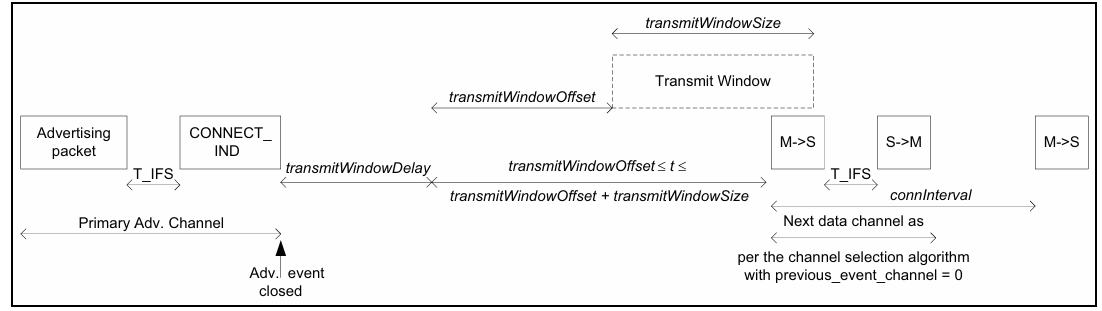
\includegraphics[width = 1\textwidth]{image/Master 連接建立過程和連接事件.png}
    \caption{Master 連接建立過程和連接事件\cite{bluetooth2016core}}
    \label{fig: Master 連接建立過程和連接事件}
\end{figure}

錨點(Anchor Point, AP)是 BLE 連線中用來做為 Master 與 Slave 雙方傳輸時間的參考點,確保雙方能在預期的時刻進行資料交換。透過錨點的設置,Slave 可以準確地進入低功耗睡眠與喚醒,達到節能與通訊準確的目的。

CONNECT\_IND封包會在 $t_{ind}$ 時間內完成傳輸,Master 會在\ref{eq: a}式至\ref{eq: b}式的時間內設置第一個錨點(Anchor Point, AP),其中 transmitWindowDelay 通常為 $1.25\,{ms}$,用來同步 Master 與 Slave。

transmitWinOffset 與 transmitWinSize 分別由\ref{eq: c}式與\ref{eq: d}式算出。WinOffset代表錨點(Anchor Point, AP)的偏移量;WinSize代表錨點(Anchor Point, AP)可能發生的時間範圍\cite{10.1145/3412382.3458271}。

\begin{equation}
t_{ind} + transmitWindowDelay + transmitWinOffset
\label{eq: a}
\end{equation}

\begin{equation}
t_{ind} + transmitWindowDelay + transmitWinOffset + transmitWinSize
\label{eq: b}
\end{equation}

\begin{equation}
transmitWinOffset = WinOffset \times 1.25\, ms
\label{eq: c}
\end{equation}

\begin{equation}
transmitWinSize = WinSize \times 1.25\, ms 
\label{eq: d}
\end{equation}

\section{藍牙網狀網路}

藍牙網狀網路(Bluetooth Mesh)是由藍牙技術聯盟(Bluetooth Special Interest Group)於2017年發布的標準,旨在解決傳統藍牙技術在物聯網(IoT)應用中的傳輸距離限制。藍牙網狀網路允許多個BLE裝置之間建立一個可靠且可擴展的網狀結構,這使得裝置之間可以進行多跳傳輸,從而擴大了傳輸距離和覆蓋範圍。

Bluetooth Mesh 是基於藍牙低功耗(Bluetooth Low Energy, BLE)的網狀網路技術,是多個裝置進行多對多(many-to-many)連接的拓樸技術,可以將資料從BLE Mesh中的其中一個節點,發送至BLE Mesh中的任何一個節點,且任兩個節點間的傳輸路徑,並不會只有一條,因為這種多重路徑(multi-path)的特性,讓Mesh中如果有一個節點故障,也不會因此癱瘓整個系統。此技術有效解決了 BLE 在長距離和多設備連接上的限制,擴展了 BLE 的應用範圍,特別適用於無線感測網路(Wireless Sensor Networks, WSN)和物聯網(IoT)環境。

Bluetooth Mesh 保有BLE的優點,並改善BLE傳輸範圍有限的問題,Bluetooth Mesh的網路架構分為 Flooding 模式及Routing 模式,Flooding Mesh 是大多數 BLE Mesh 協定採用的傳輸模式,利用廣播方式傳送訊息,無需建立節點間的連接,節點將訊息以廣播模式傳遞給通訊範圍內的所有節點,節點收到訊息後再次廣播,直到訊息傳遞至目標節點為止。

Routing Mesh 使用連接模式,節點需在訊息傳輸前建立節點間的連接,確保訊息傳遞有序且可靠。節點之間先建立連接,資料通過預設路徑逐步傳遞至目的節點,並根據需求動態調整路由,因為資料傳輸通過固定路徑,減少碰撞和干擾,讓傳輸更穩定。也因為訊息傳遞通過固定的路徑,降低重複廣播次數,節省了不必要的電能消耗。Routing Mesh 資料傳輸的方式確保資料完整傳遞,即使網路繁忙也能正常運作。相對的缺點也顯而易見,因為資料傳遞時,節點間需建立連接,設計上比較複雜而增加實現難度。且建立連接需耗費額外時間,當路徑上的節點完成所有連接後才會開始傳輸,所以網路啟動比較慢。也會因為接點間連接路徑較長,讓資料傳遞時間增加,最後產生較高的傳輸延遲。

\section{分時多工與BLE中的CI與CE機制}

分時多工 (Time Division Multiple Access, TDMA) 如字面上的意義,它一種將時間分割的通訊技術,讓多個裝置可以高效的共享同一傳輸介質進行傳輸。TDMA 將時間劃分為多個時槽 (Time Slots),每個裝置只能在指定的時槽內進行傳輸,這確保了同一時刻,只有一個裝置進行傳輸,其他的裝置在同一個時間下(相同Time slot),都處於等待的狀態,可以確保訊號穩定且不重疊,有效避免了訊號重疊和干擾而導致的數據丟失。

在BLE中,TDMA的理念被具體實現在連線模式下的CI與CE設計中。BLE通訊雙方在建立連線後,會協商出一個固定的CI,作為接下來通訊週期的基本單位。每個CI之內,雙方僅在特定的CE中進行資料交換,其餘時間則處於睡眠或非活躍狀態。

這樣的設計與TDMA的概念密切相關:每個BLE連線設備實際上都在預定的時槽(即CE時間內)進行資料交換,彼此間在時間上分離,以避免干擾與資源衝突。尤其在多裝置共存環境中,例如一個主裝置(Central)與多個從裝置(Peripheral)連線時,主裝置會根據各連線的CI設計,輪流與不同的裝置進行資料交換,實現一種類似TDMA的排程與存取控制機制。

\section{目的地傾向傳輸}

FruityMesh是一個專門為BLE Mesh Network所開發的開源連接模式之網路協定,在 FruityMesh 的傳輸機制中,訊息從一個節點發送至中繼節點時,中繼節點會廣播訊息給所有相鄰節點,相鄰的節點又會在廣播給其相鄰的節點,直到目標節點,而廣播風暴會造成節點間多餘不必要的資料傳輸,而增加網路的負擔。為了解決廣播風暴問題,目的地傾向傳輸(Destination-Oriented Transmission, DOT)\cite{112TIT00392032}機制,通過引入方向性和目的傾向的傳輸策略,優化封包的傳輸過程,減少網路負載與封包重傳,提升傳輸效率與穩定性。

DOT 機制利用樹狀架構中的 Level 層級概念,在假設封包都是以根(Root)節點為目的端的前提下,為每個節點計算其所屬層級,使用 FIND\_LEVEL 封包進行層級標記,而根節點的Level值最低,傳輸方向封包只需傳遞至 Level 較低 的節點,避免無意義的廣播。DOT 在中繼節點限制封包的傳輸方向,僅向 Level 較低的節點傳輸封包,這種方式有效減少了網路流量,降低碰撞率,並提升了傳輸可靠性。

\section{目的地傾向切換傳輸}

目的地傾向切換傳輸(Destination Oriented Switch Transmission, DOST)\cite{112TIT00392032}機制進一步解決角色身份重疊與傳輸重疊的問題,通過啟用與禁用連線的方式,降低網路負載並避免封包重傳,解決BLE網狀網路節點可能因同時扮演Master和Slave角色衝突而導致的封包傳輸遺失現象。

在啟用與禁用功能的運作中,節點傳輸 INIT\_STATE 封包,用於標記和控制各連線的啟用或禁用狀態,確保所有節點對於連線的處理具有一致性,節點在某一連線傳輸封包時,禁用其他連線以避免通訊重疊,每個 Connection Interval 結束後,切換連線的啟用與禁用狀態,雖然可能導致封包延遲一個 Connection Interval,但有效降低了網路負載,提升傳輸效率,如圖\ref{fig: 傳輸機制的節點時序示例}所示。

\begin{figure}[H]
    \centering
    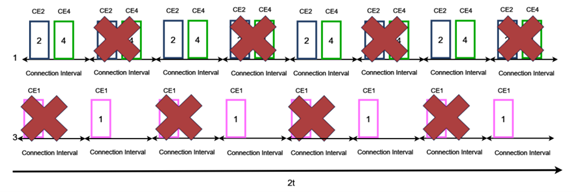
\includegraphics[width = 0.8\textwidth]{image/傳輸機制的節點時序示例.png}
    \caption{傳輸機制的節點時序示例\cite{112TIT00392032}}
    \label{fig: 傳輸機制的節點時序示例}
\end{figure}

\section{Nordic Semiconductor nRF52840}
nRF52840 是 nRF52 系列中很先進的成員,專為應對需要協定並行處理和複雜應用挑戰的需求而設計。它提供充裕的快閃記憶體與 RAM 空間,能滿足高性能應用的需求。
nRF52840 支援多協定並行運作,包含低功耗藍牙、藍牙 Mesh 網狀網路、Thread、Zigbee、IEEE 802.15.4、ANT 及 2.4 GHz 專有協定,讓其在多種應用場景中均表現出色。

此 SoC 採用 32 位元 ARM® Cortex™-M4 處理器,具備浮點運算單元,主頻達 64 MHz。內建 NFC-A 標籤,可簡化裝置配對或用於支付應用。此外,晶片搭載 ARM TrustZone® CryptoCell 安全加密單元,能在 CPU 之外高效處理加密演算法,提供強大的安全性。

nRF52840 也整合多種數位周邊和介面,包括高速 SPI 與 QSPI,能連接外部快閃記憶體與顯示裝置;PDM 與 I2S 接口用於連接數位麥克風與音訊設備。此外,內建全速 USB 控制器,支援資料傳輸功能,亦可作為電池充電的電源來源。

透過先進的片上自適應電源管理系統,nRF52840 實現了極低功耗,適合各類高效能且低能耗的應用需求,所以選用Nordic Semiconductor的nRF52840-DK開發板\cite{nordic2023softdevices}作為本次的硬體設備,如圖\ref{fig: nRF52840-DK開發板}所示
。

\begin{figure}[H]
    \centering
    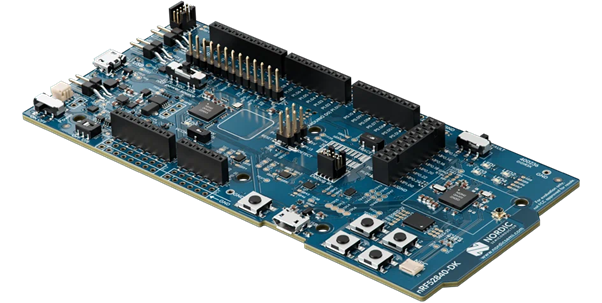
\includegraphics[width = 0.8\textwidth]{image/nRF52840-DK開發板.png}
    \caption{nRF52840-DK開發板}
    \label{fig: nRF52840-DK開發板}
\end{figure}

\section{FruityMesh開發平台介紹}
FruityMesh \cite{fruitymesh2023} 專為 BLE Mesh Network設計的開源通訊協定框架。該平台主要針對 Nordic Semiconductor 所推出之 nRF52 系列晶片(例如 nRF52832、nRF52840)進行最佳化,提供節點之間低功耗、穩定且具擴展性的無線通訊能力,廣泛應用於物聯網(IoT)場景。

FruityMesh 架構底層結合 Nordic SoftDevice 的藍牙堆疊,搭配即時任務管理與連線資源控管模組,能夠有效分配 Mesh 內部的連線插槽(Connection Slots)與角色權限。此外,其內建的 Clustering 與 Routing 機制可支援點對點封包傳遞與多跳路由(Multi-hop),達成資料有效分散與收斂的設計目標。

本研究即基於 FruityMesh 為開發基礎,進一步修改其拓樸建立、排程控制、連線優化與自我修復(Self-Healing)機制,以因應實際多節點部署中所可能遭遇的延遲、壅塞與節點斷線等問題。

\subsection{Nordic SoftDevice}
SoftDevice 是由 Nordic Semiconductor \cite{nordic2023softdevices} 提供的一組 預編譯、經過認證 的無線通訊定堆疊 (Protocol Stack),專為nRF系列(如nRF52840、nRF52832)等Bluetooth Low Energy(BLE)與ANT無線晶片設計。SoftDevice主要負責BLE 通訊協定的完整實作,並且以軟體庫的形式提供,方便嵌入式開發者在不需理解底層協定的情況下進行無線應用開發。

\subsection{FruityMesh Cluster}
在 FruityMesh \cite{fruitymesh2023} 架構中,Cluster(叢集)機制扮演了關鍵的角色。該機制允許網路中的節點根據功能或地理位置進行分組,以降低整體網路中不必要的廣播與封包重傳,進而提升通訊效率與穩定性。每個 Cluster 可被視為一個子網,其內部節點之間擁有穩定的連線關係,並可視需求與其他 Cluster 建立通訊橋接,使整體網路具備良好的可擴展性與模組化管理能力。

當一個節點首次啟動時,會主動進入 High Discovery 狀態,並開始廣播 JOIN 封包以尋找可連接的節點。隨著時間推進,鄰近節點會逐步聚合形成數個 Cluster,並根據連線策略逐步合併成為一個完整的網狀結構。在 FruityMesh 的預設演算法中,節點在選擇連線對象時會優先考量 Cluster 的節點數量,傾向加入節點較多的 Cluster。因此,整體網路會自然形成「大 Cluster 併吞小 Cluster」的現象,最終形成一個包含所有節點的 Spanning Tree 拓樸結構。

\subsection{FruityMesh Self-Healing}
為強化網路穩定性,FruityMesh \cite{fruitymesh2023} 同時設計了 Self-Healing(自我修復)機制。當網路中某個節點因掉電、移動或干擾等原因導致斷線,系統會自動啟動恢復流程。具體而言,斷線的節點會立即廣播連線請求封包至其通訊範圍內的所有鄰近節點。一旦鄰近節點接收到該封包,便會與之進行連線協商程序,使該孤立節點得以重新加入原有網路拓樸中。

此機制基於 FruityMesh 支援的多跳傳輸設計,確保即使部分節點失效,網路仍可自動尋找可行的替代路徑傳遞資料。Self-Healing 機制大幅提升了 BLE Mesh 系統在實際部署環境中的容錯性與可靠性,亦減少了人工維護與手動重連的需求,對於物聯網應用中的大規模部署具有重要意義。

\end{ZhChapter}
% 章節三 Chapter 3
\begin{ZhChapter}

\chapter{BLE Mesh拓樸建立機制設計}

\section{問題分析}

\subsection{BLE Mesh拓樸建立問題}

在原生FruityMesh架構中,節點的建立與連線並未針對資料匯集或匯出端進行特別設計,因此整體網路並無明確的Root節點。其封包傳輸方式主要採用廣播機制,即每當節點產生封包時,會向所有相鄰節點廣播傳送,期望藉由鄰近節點的重傳將封包推進至目的地。雖然此方法具備一定的自我修復能力,但在多節點、大範圍的Mesh網路中,極易導致封包重複傳送與碰撞,進而產生所謂的「廣播風暴」現象,嚴重影響整體網路效能與穩定性。

為了解決此問題,\cite{112TIT00392032}研究中引入DOT機制,將原先的無向廣播傳輸改為目的導向的封包路由方式,透過樹狀拓樸的建立使資料傳輸路徑更具方向性與效率性。然而,導入DOT排程機制的前提之一,是整個BLE Mesh網路需具備清楚的階層結構,而Sink節點(資料匯集端)必須作為整體樹狀拓樸的根節點。唯有如此,封包才能沿著既定的父子節點路徑,自節點有效匯流至Sink節點,達成DOT排程所需的單向、無冗餘傳輸目標。

然而,由於FruityMesh原生設計並非以Sink節點為中心的拓樸為出發點,現有拓樸建立流程尚無法保證Sink節點必然成為根節點。在未進行拓樸控制調整的情況下,可能出現Sink位置處於樹葉節點甚至中繼節點等非理想情境。因此,若要在FruityMesh架構中有效實作DOT排程機制,勢必需重新設計拓樸建立邏輯,強制指定使Sink節點始終位於拓樸樹的根部,即使在斷線並重新連線的情況下,亦能恢復其根節點角色,確保網路穩定性與傳輸效能。

\subsection{BLE Mesh封包傳輸問題}

在基於FruityMesh的藍牙低功耗網狀網路傳輸機制設計中,\cite{112TIT00392032}研究已針對封包延遲與封包抵達率等品質指標進行優化,並取得初步成效。該研究藉由導入DOT與DOST排程機制,成功改善了大部分的傳輸延遲與資料完整性。然而,即使在優化機制下,網路中仍不時出現封包遺失(掉封包)與重傳現象,顯示目前的傳輸機制尚存在進一步提升的空間。

造成封包掉落與重傳的關鍵因素之一,在於BLE Mesh網路的流量集中特性。由於整體網路皆以Sink節點作為封包的最終目的地,所有資料封包最終皆會匯集至該節點,導致越接近Sink的節點需承擔更多的中繼與轉發任務。這種負載不均的現象將使中樞節點在短時間內接收到大量傳輸要求,導致中樞節點的Sent buffer資源迅速耗盡。一旦緩衝區爆滿,不僅無法即時處理新進封包,還可能造成排程延遲、封包掉落,進而引發重傳機制啟動,進一步加重網路負載。

為有效緩解此類壅塞現象,需從連線參數層級進行調整,特別是針對CI與CE進行優化配置。透過適當調整CI間隔,可有效控制節點可傳輸封包的節奏與頻寬分配,進一步降低高負載節點的壓力,提升整體封包處理效率。結合連線參數調整機制,可以有效改善封包壅塞問題,以提升BLE Mesh網路在多節點、高流量情境下的服務品質。

\clearpage

\section{BLE Mesh拓樸建立機制設計}

本論文提出改善FruityMesh的拓樸建立機制,確保Sink節點始終位於整體網路的根節點,並在斷線後能夠自動恢復其角色。此設計為後續的DOT排程機制提供穩定的基礎,如圖\ref{fig: 提出的拓樸建立流程圖}所示。

圖\ref{fig: 提出的拓樸建立流程圖}中也針對有底色的部分進行修改,可以更加確保Sink節點始終位於整體網路的根節點,如Algorithm \ref{alg: CalculateClusterScoreAsMaster} 及 Algorithm \ref{alg: CalculateClusterScoreAsSlave}所示。

\begin{figure}[H]
    \centering
    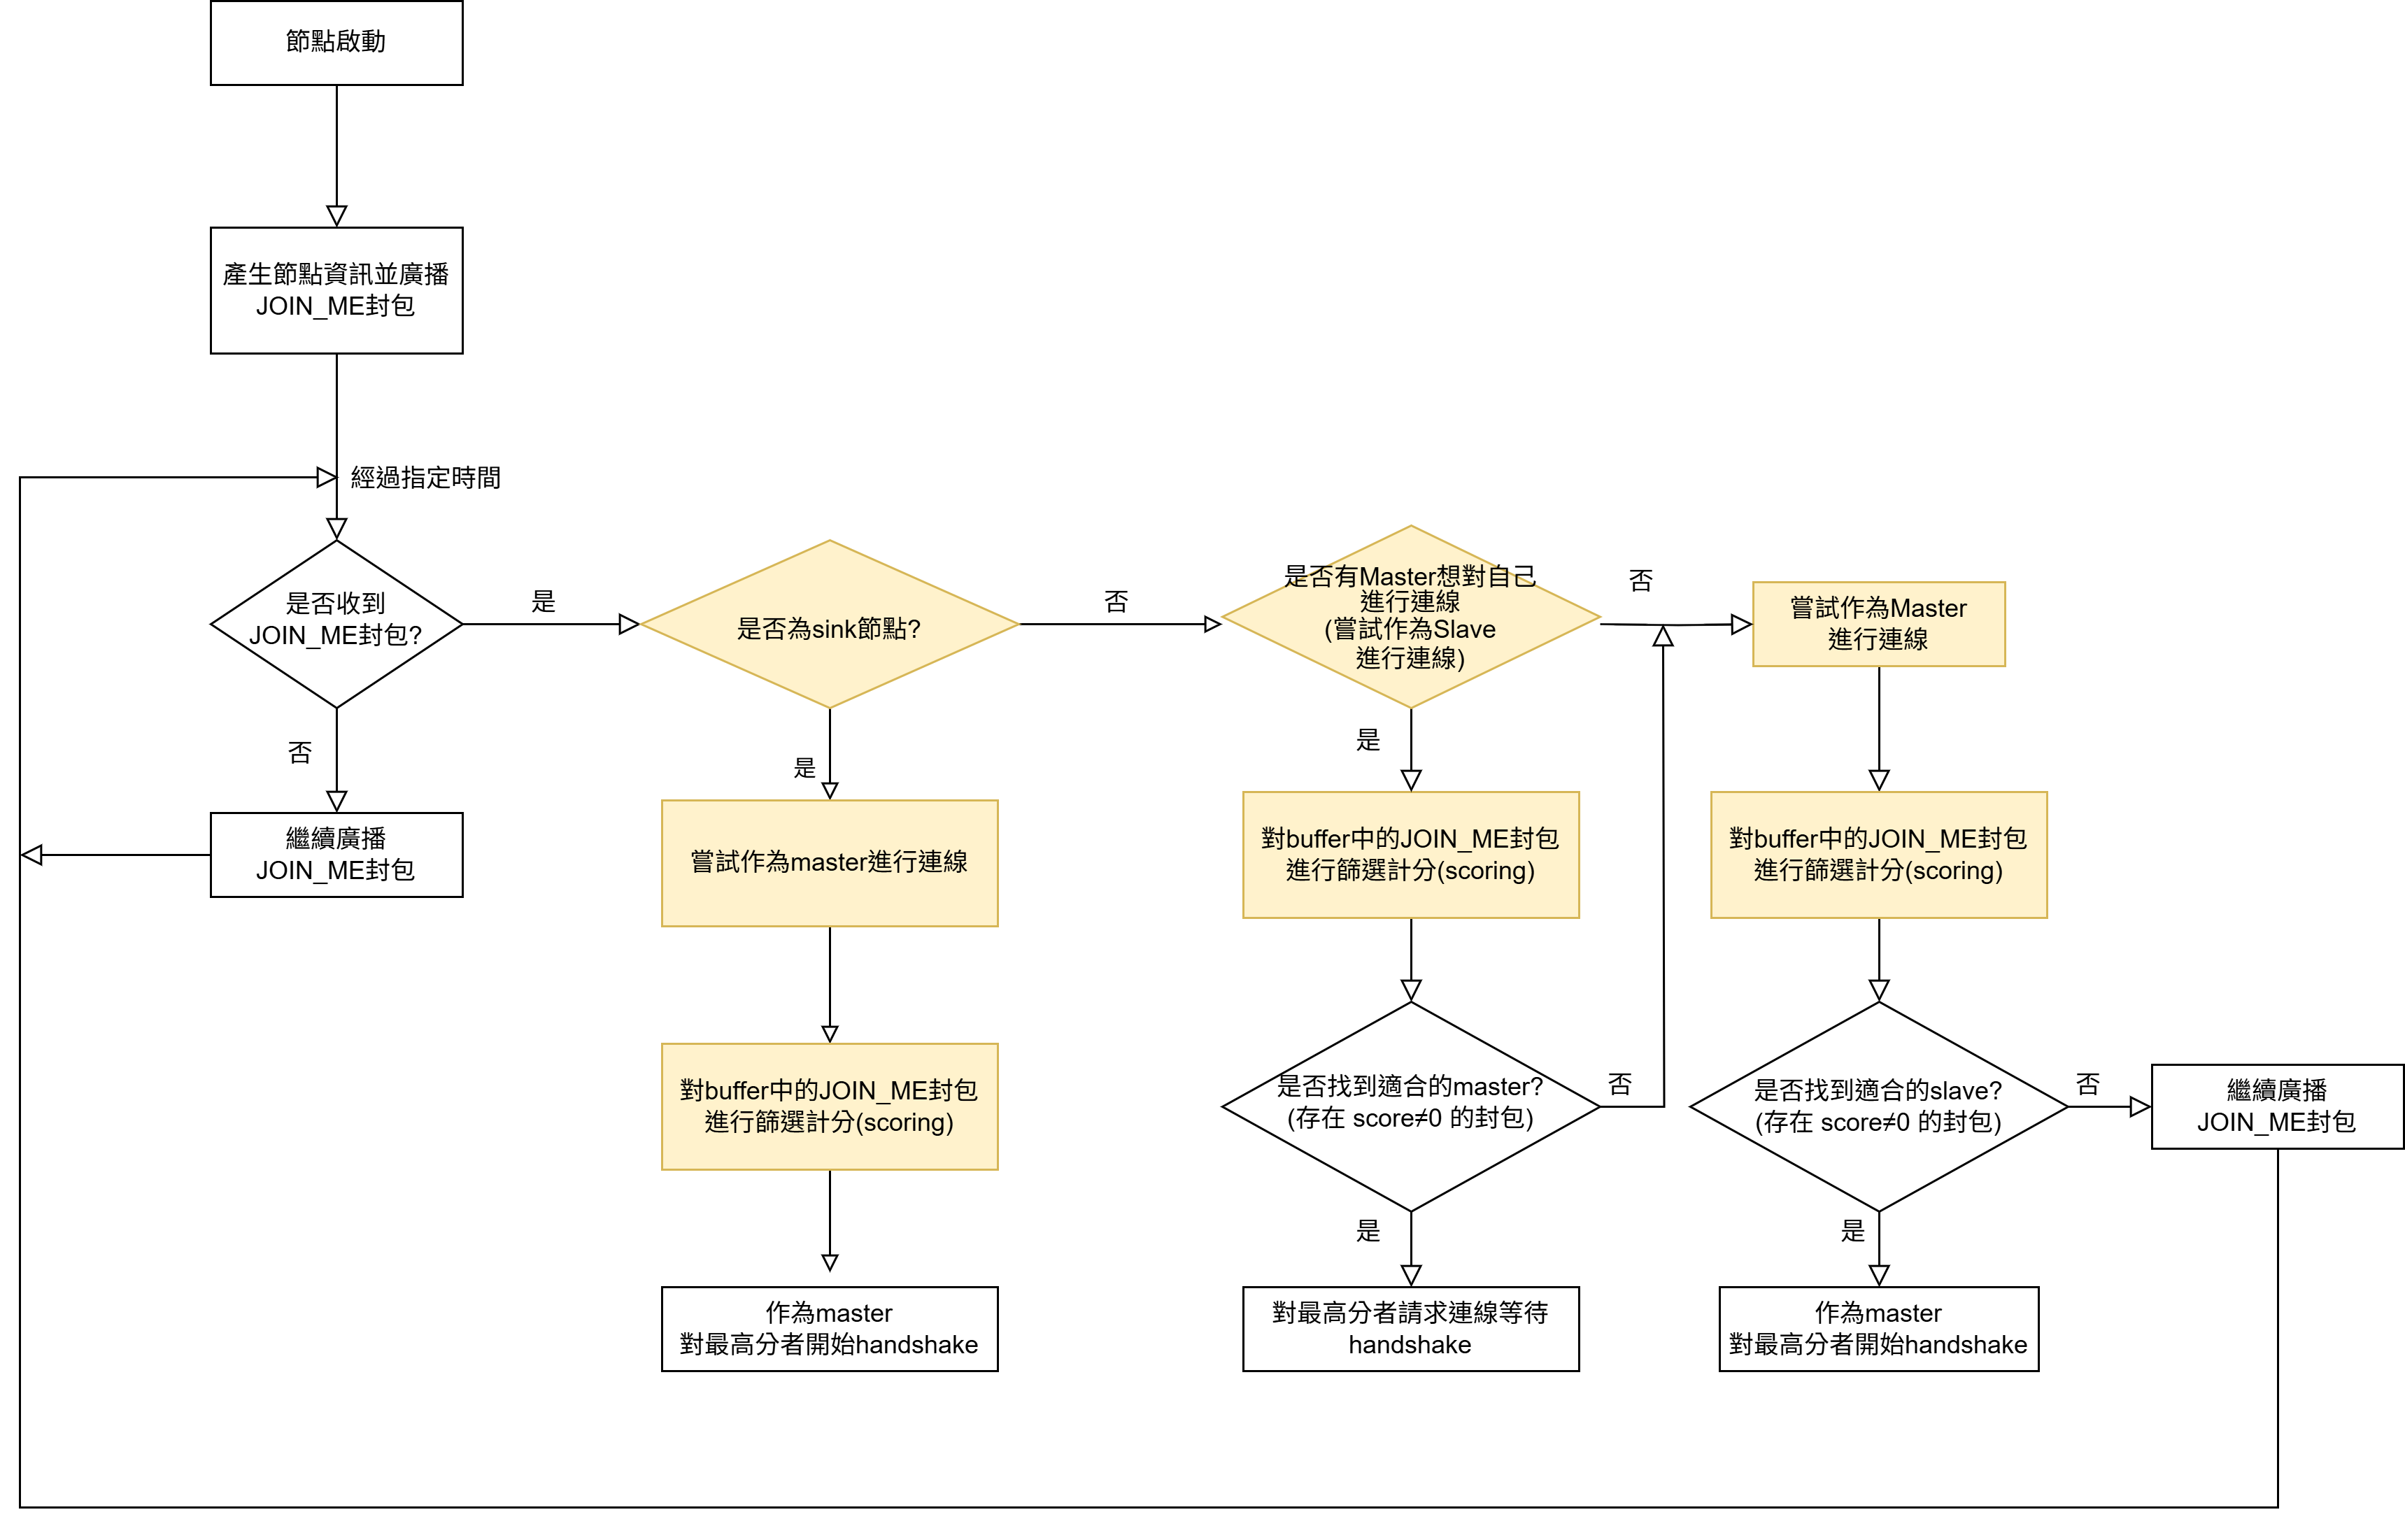
\includegraphics[width = 1\textwidth]{image/build-up_pro2.png}
    \caption{提出的拓樸建立流程圖}
    \label{fig: 提出的拓樸建立流程圖}
\end{figure}

在拓樸建立流程啟動時,每個節點在開機後會廣播包含自身節點資訊的JOIN\_ME封包。節點收到其他節點所廣播的JOIN\_ME封包後,會將該封包儲存於本地緩衝區中,並根據封包內容進行評分(scoring),以評估對方作為連線對象的適合程度。此評分機制可根據鄰近程度、RSSI訊號強度、是否為Sink節點等參數進行加權計算,從而判斷潛在連線對象的優先順序。

若節點本身為預先指定的Sink節點,則會主動嘗試以Master的角色發起連線,以確保其成為拓樸的根節點。另一方面,對於非Sink節點,為了確保拓樸架構的根節點為Sink節點,節點在評估過程中會優先以Slave身分尋找合適的Master進行連線。只有當未能找到合適的Master節點(例如評分皆為0或未收到有效的JOIN\_ME封包)時,該節點才會轉而作為Master嘗試連線至其他尚未建立連線的節點,進一步擴展網路的拓樸結構。

若節點在轉為Master之後,仍未能找到合適的Slave節點(即緩衝區中所有JOIN\_ME封包的評分皆為0或無法建立穩定連線)時,該節點將回到初始狀態,繼續定期廣播JOIN\_ME 封包,以等待後續更合適的連線機會出現。此重試機制能避免節點因短期內找不到連線對象而陷入孤立狀態,提升整體拓樸建立的成功率與網路的自組織能力。

\subsection{決定最好的群組加入}

Algorithm \ref{alg:determine_best_cluster_part1}及Algorithm \ref{alg:determine_best_cluster_part2}及Algorithm \ref{alg:determine_best_cluster_part3}描述了節點在藍牙低功耗網狀網路(BLE Mesh)中,決定其與其他節點建立連線方式的邏輯流程。其核心目標是依據當下網路狀態與節點角色,判斷該節點應該主動發起連線(作為Master)或是被動接受連線(作為Slave)。

\begin{algorithm}[H]
\caption{DetermineBestClusterAvailable - Part 1}
\label{alg:determine_best_cluster_part1}
\begin{algorithmic}[1]
\State Initialize \texttt{result} as \texttt{NO\_NODES\_FOUND}
\State Get device type and assign to \texttt{deviceType}
\If{deviceType is \texttt{SINK} and outbound connections are available}
    \State \texttt{bestClusterAsMaster} $\gets$ \texttt{DetermineBestClusterAsMaster()}
    \If{\texttt{bestClusterAsMaster} $\neq$ null}
        \State Adjust \texttt{connectionIv} based on peer’s device type
        \State Attempt to connect as Master
        \If{connection succeeds}
            \State Update connection attempt time and count
        \EndIf
        \State Set \texttt{result.result} $\gets$ \texttt{CONNECT\_AS\_MASTER}
        \State Set \texttt{result.preferredPartner} $\gets$ bestClusterAsMaster.sender
        \State \Return result
    \EndIf
\EndIf
\end{algorithmic}
\end{algorithm}

Algorithm \ref{alg:determine_best_cluster_part1}流程一開始會檢查當前節點是否為SINK且具備可用的對外連線資源。若節點為Sink節點,則優先考慮作為Master嘗試連線,並透過DetermineBestClusterAsMaster()函式選出最合適的連線目標節點。若成功取得候選節點,系統會根據對方裝置的類型調整連線參數(如CI),並嘗試建立連線。若連線成功,系統會更新連線時間與次數統計,並回傳連線成功的決策結果。

\begin{algorithm}[H]
\caption{DetermineBestClusterAvailable - Part 2}
\label{alg:determine_best_cluster_part2}
\begin{algorithmic}[1]
    \State Reset \texttt{currentAckId} to 0
    \State \texttt{bestClusterAsSlave} $\gets$ \texttt{DetermineBestClusterAsSlave()}

    \If{deviceType is \texttt{SINK}}
        \State \texttt{bestClusterAsSlave} $\gets$ null
    \EndIf

    \If{\texttt{bestClusterAsSlave} $\neq$ null}
        \State \texttt{currentAckId} $\gets$ bestClusterAsSlave.clusterId
        \If{\texttt{meshMaxInConnections == 1}}
            \State Check if any fresh connection exists (handshake not expired)
            \If{no fresh connection and \texttt{freeMeshInConnections == 0}}
                \If{clusterSize $\neq$ bestClusterAsSlave.clusterSize OR random trigger passed}
                    \State Force disconnect other mesh connections
                    \State Reset cluster size to 1
                    \State Generate new \texttt{clusterId}
                \EndIf
            \EndIf
        \EndIf
        \State Update JoinMe packet
        \State Set \texttt{result.result} $\gets$ \texttt{CONNECT\_AS\_SLAVE}
        \State Set \texttt{result.preferredPartner} $\gets$ bestClusterAsSlave.sender
        \State \Return result
    \EndIf
\end{algorithmic}
\end{algorithm}

Algorithm \ref{alg:determine_best_cluster_part2}為若節點角色並不是Sink節點,則會優先作為Slave接受他人連線。此時會重設回應欄位(currentAckId),並透過DetermineBestClusterAsSlave()選出合適的候選節點。並再次檢查當前節點如果為SINK節點,則不允許Sink節點作為Slave進行連線。當節點作為Slave進行連線時,若符合條件的Master節點存在,系統則會建立連線。

\begin{algorithm}[H]
\caption{DetermineBestClusterAvailable - Part 3}
\label{alg:determine_best_cluster_part3}
\begin{algorithmic}[1]
\State \texttt{bestClusterAsMaster} $\gets$ \texttt{DetermineBestClusterAsMaster()}
\If{\texttt{bestClusterAsMaster} $\neq$ null and outbound connections are available}
    \State Adjust \texttt{connectionIv} and attempt to connect
    \If{connection succeeds}
        \State Update connection info
    \EndIf
    \State Set \texttt{result.result} $\gets$ \texttt{CONNECT\_AS\_MASTER}
    \State Set \texttt{result.preferredPartner} $\gets$ bestClusterAsMaster.sender
    \State \Return result
\EndIf

\State Log `no cluster found'
\State Set \texttt{result.result} $\gets$ \texttt{NO\_NODES\_FOUND}
\State \Return result
\end{algorithmic}
\end{algorithm}

Algorithm \ref{alg:determine_best_cluster_part3}為當節點作為Slave進行連線沒有找到適合的Master時,則該節點會再度嘗試以Master身分建立連線,重複執行候選節點評估與連線流程,若成功,則回傳連線結果。最後如果所有嘗試皆沒有辦法成功連線,系統會記錄「未找到叢集」的訊息,並回傳 NO\_NODES\_FOUND 的決策結果。

\subsection{以Mater身分選擇最佳的Slave}

\begin{algorithm}[H]
\caption{CalculateClusterScoreAsMaster}
\label{alg: CalculateClusterScoreAsMaster}
\begin{algorithmic}[1]
\State Retrieve device type from device configuration
\If{packet is too old} \Return 0 \EndIf
\If{packet.clusterId == this.clusterId} \Return 0 \EndIf
\If{packet has no free inbound connections} \Return 0 \EndIf
\If{packet.ackField $\neq$ this.clusterId and $\neq$ 0} \Return 0 \EndIf
\If{packet.clusterSize $>$ current cluster size \textbf{and} current device is not SINK} \Return 0 \EndIf
\If{packet is temporarily blacklisted} \Return 0 \EndIf
\If{already connected to packet.sender} \Return 0 \EndIf
\If{packet.rssi $<$ threshold} \Return 0 \EndIf
\If{current device type == LEAF} \Return 0 \EndIf

\State $rssiScore \gets 100 + packet.rssi$
\State $score \gets packet.freeMeshOutConnections + rssiScore$
\State Modify score using preferred partner policy
\State \Return score
\end{algorithmic}
\end{algorithm}

Algorithm\ref{alg: CalculateClusterScoreAsMaster}說明了節點在嘗試成為Master時,如何針對鄰近的叢集候選節點進行評分。該評分機制用來決定是否值得主動與某個節點建立連線。

一開始,節點會先取得自身的裝置類型,若為LEAF(葉節點)則無法發起連線,直接回傳0分。
接著系統會篩選掉以下不合適的候選節點:

\begin{itemize}
    \item 候選節點的封包太舊
    \item 與候選節點的叢集相同
    \item 候選節點無inbound connections的數量可以使用
    \item 與候選節點的ack欄位不符
    \item 候選節點不是Sink節點且對方叢集較大
    \item 候選節點在短時間內已多次連線失敗(暫時黑名單)
    \item 已與該節點連線中
    \item 候選節點的RSSI過低
\end{itemize}

若符合條件,則將計算RSSI分數,並依據以下項目計算總分:
\begin{itemize}
    \item 候選節點的freeMeshOutConnections數量。
    \item 實際RSSI品質分數(rssiScore)。
\end{itemize}

該分數越高,代表候選節點作為目前節點選擇最佳 Slave 的依據,最後,還會根據偏好節點(preferred partner)進行微調後,回傳最終評分結果。

\subsection{以Slave身分選擇最佳的Master}

\begin{algorithm}[H]
\caption{CalculateClusterScoreAsSlave}
\label{alg: CalculateClusterScoreAsSlave}
\begin{algorithmic}[1]
\State Retrieve device type from configuration
\If{deviceType == SINK} \Return 0 \EndIf
\If{packet.hopsToSink < 0} \Return 0 \EndIf
\If{packet.freeMeshOutConnections == 0} \Return 0 \EndIf
\If{packet is too old} \Return 0 \EndIf
\If{packet.clusterId == current.clusterId} \Return 0 \EndIf
\If{packet.clusterSize < current cluster size \textbf{and} packet.deviceType $\neq$ SINK} \Return 0 \EndIf
\If{packet.rssi < threshold} \Return 0 \EndIf

\State $rssiScore \gets 100 + packet.rssi$
\State $score \gets 0$
\If{packet.deviceType == SINK}
    \State $score \gets score + 10000$
\EndIf

\State $score \gets score + (packet.clusterSize \times 100) + (packet.freeMeshOutConnections \times 100) + rssiScore$
\State Modify score based on preferred partner logic
\State \Return score
\end{algorithmic}
\end{algorithm}

Algorithm\ref{alg: CalculateClusterScoreAsSlave}描述了節點在考慮作為 Slave 加入其他叢集時,如何針對潛在的 Master 節點進行評分。

首先系統會排除不適合的情況:
\begin{itemize}
    \item 若目前節點為SINK節點,則無法作為Slave加入其他叢集。
    \item 候選節點的hopsToSink小於0。
    \item 候選節點無freeMeshOutConnections的數量可以使用。
    \item 候選節點的封包太舊。
    \item 當前節點與候選節點為同一叢集。
    \item 候選節點並非SINK節點且候選節點叢集規模小於當前節點叢集。
    \item 候選節點的RSSI過低。
\end{itemize}

若符合條件,則將計算RSSI分數,並依據以下項目計算總分:

\begin{itemize}
    \item 候選節點是否為SINK節點,若是Sink節點會獲得額外的10000分。
    \item 對方叢集大小(clusterSize)乘以100。
    \item 可用的 freeMeshOutConnections 數量乘以100。
    \item 實際 RSSI 品質分數(rssiScore)
\end{itemize}

最終分數會再次根據偏好節點機制進行修正,分數最高代表候選節點作為目前節點最佳 Master 的依據。


\subsection{Self-Healing機制的拓樸修復改進}

原生FruityMesh提供了Self-Healing機制,使節點在斷線後能回到HIGH\_DISCOVERY狀態並尋找可連線的鄰居節點,且會由小的叢集合併進大的叢集,從而重新建立連線。然而,此機制下若斷線的是Root(Sink)節點,重新連回後將失去Root身份,可能導致整個網路拓樸失效或性能下降。

為解決此問題,本研究修改了CLUSTER\_WELCOME訊息的握手流程。在握手判斷邏輯中,若發現對方為SINK且其Cluster比自己小(或等於),則避免讓原本為Root的節點退位為普通節點,並強制原Cluster切斷其他連線,重新啟動拓樸建立,使原本的SINK節點能保有Root身份,維持拓樸穩定性與網路一致性,如Algorithm\ref{alg: Topology Self-Healing Handshake Logic}所示。

\begin{algorithm}[H]
\caption{Topology Self-Healing Handshake Logic}
\label{alg: Topology Self-Healing Handshake Logic}
\begin{algorithmic}[1]
\Require CLUSTER\_WELCOME packet received
\If{packet size invalid}
    \State Log and ignore packet
\Else
    \State Save partner handle and enter HANDSHAKING state
    \State Backup local cluster ID and size
    \If{remote cluster ID == local cluster ID}
        \State Disconnect: SAME\_CLUSTERID
    \ElsIf{remote cluster size < local size \textbf{and} remote is not SINK}
        \If{connection is inbound}
            \State Disconnect: WRONG\_DIRECTION
        \EndIf
    \ElsIf{network ID mismatch}
        \State Disconnect: NETWORK\_ID\_MISMATCH
    \ElsIf{connection is not preferred \textbf{and} preferences ignored}
        \State Disconnect: UNPREFERRED\_CONNECTION
    \Else
        \State Accept connection as Root
        \State Send CLUSTER\_ACK\_1 with hopsToSink = 0 if self is SINK
        \State Disconnect all other mesh connections
        \State Reinitialize local cluster with size = 1 and new ID
    \EndIf
\EndIf
\end{algorithmic}
\end{algorithm}

Algorithm\ref{alg: Topology Self-Healing Handshake Logic}為了強化FruityMesh在節點斷線重連後的拓樸穩定性,本研究在原有 Self-Healing機制之上,進一步修改其握手邏輯。當節點收到 CLUSTER\_WELCOME 封包後,將進入拓樸重組的判斷流程。具體邏輯如下:

\begin{itemize}
    \item 首先,節點會確認封包的大小是否正確,若不正確則忽略該封包。
    \item 接著,進入Handshaking狀態並備份目前的Cluster ID與Cluster大小,用以後續比對使用。
    \item 若對方節點的Cluster ID與自己相同,代表已屬同一個Cluster,這在初始階段是不應該出現的情況,因此直接斷線處理。
    \item 若對方的 Cluster大小比本地端小,且其並非SINK節點,則本節點認定自己應作為主導方,若該連線是inbound,則代表方向錯誤,同樣會中止連線。
    \item 若兩節點的network ID不一致,或連線對象並非偏好的節點,也將被強制中止以避免不必要的Mesh錯誤連線。
\end{itemize}

在以上檢查皆通過的情況下,代表本節點應接受對方節點加入自己的 Cluster。若本節點為SINK節點,則會在 CLUSTER\_ACK\_1 回覆中指定 hopsToSink = 0,表明自己為Mesh根節點,並強制中斷其他 Mesh連線,重新以自己為中心建立拓樸結構,確保在重新連線的情況下仍能維持SINK節點的Root地位。

\section{BLE Mesh封包傳輸機制設計}
在 BLE Mesh 網路中,封包傳輸的效率與穩定性對整體系統效能具有關鍵影響。尤其在具備多跳(multi-hop)特性的網狀架構中,位於拓樸上層的節點(例如接近 Root 的節點)需承擔來自下層節點的大量封包轉送任務,因此其封包處理壓力遠高於葉節點。

若未妥善配置這些節點的傳輸參數,將容易造成 sent buffer 過載、傳輸延遲增加、甚至出現頻繁重傳等問題,進而影響整體系統穩定性與效能表現。

為了改善上述問題,本研究提出一種基於節點層級調整連線間隔參數(Connection Interval, CI)的機制,如圖 \ref{fig: BLE Mesh封包傳輸機制設計節點架構圖} 所示。設計理念為:根據節點於拓樸中的層級深度,賦予不同的 CI 值,越靠近 Root 的節點,其連線間隔設定越短,以提供更頻繁的傳輸機會。此方法能夠有效緩解中繼節點所面臨的頻寬壓力,減少傳輸阻塞與重傳情形,進一步提升整體 BLE Mesh 網路的穩定性與資料傳遞效率。

\begin{figure}[H]
    \centering
    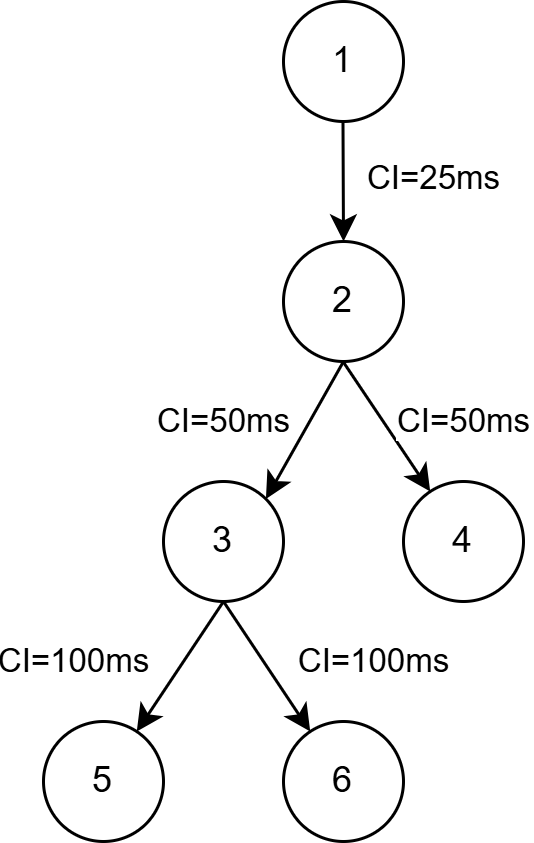
\includegraphics[width = 0.3\textwidth]{image/BLE Mesh封包傳輸機制設計節點架構圖.png}
    \caption{BLE Mesh封包傳輸機制設計節點架構圖}
    \label{fig: BLE Mesh封包傳輸機制設計節點架構圖}
\end{figure}

圖 \ref{fig: BLE Mesh封包傳輸機制設計節點架構圖} 顯示一個包含六個節點的 Mesh 拓樸,其中節點 1 為 Root。依據拓樸深度,每層的 CI 設定分別為 25 ms、50 ms 與 100 ms,形成由上而下頻率遞減的調整策略,有效反映節點所承擔的資料轉發負載,透過此層級化的參數配置機制,本研究期望在不增加硬體資源的前提下,提升多跳 BLE Mesh 網路在長時間運行中的穩定性與封包抵達率。

\end{ZhChapter}
% 章節四 Chapter 4
\begin{ZhChapter}

\chapter{實驗結果與分析}

\section{研究背景}

在本章節中,我們將介紹實驗的設計、執行過程以及結果分析。實驗旨在評估我們提出的改進方案在藍牙網狀網路(Bluetooth Mesh)中的效能,特別是在封包傳輸延遲、重傳率和整體吞吐量方面的表現。



\end{ZhChapter}
% 章節五 Chapter 5
\begin{ZhChapter}

\chapter{結論與未來工作}

\section{結論}
本研究旨在針對 FruityMesh 架構進行拓樸控制與傳輸機制的優化設計,特別著重於支援 DOT(Destination-Oriented Transmission)機制所需的拓樸先決條件,即需保證 Sink 節點始終作為整個 Mesh 網路的根節點。為此,本研究提出一套拓樸重建演算法並進行系統性模擬與實作驗證,以評估其可行性與效能。

首先,在拓樸控制部分,本研究透過模擬大規模藍牙 Mesh 網路的初始化流程,驗證所提出之拓樸重構機制可於各種隨機拓樸環境下成功將 Sink 節點設為 Mesh 網路的根節點。此外,亦模擬 Sink 節點於斷線後重新連入網路的情境,證明即使在動態變化環境下,該節點仍可重新成為根節點,維持 DOT 機制運作所需的結構一致性。雖然所提出機制在拓樸重建所需時間上略高於原生 FruityMesh,惟可提供更穩定與具控制性的網路結構,提升後續傳輸機制的可控性與預測性。

在傳輸效能方面,透過比較 HopsToSink 指標,實驗結果顯示本研究提出之拓樸機制在大多數情境下皆能有效縮短節點至 Sink 的跳數路徑,形成更平衡的 Mesh 結構,進而有助於資料傳輸效率的提升。

進一步於小規模實體環境中實作驗證,實驗亦證實在實際 BLE Mesh 網路中,無論在初始化或 Sink 斷線重連後,均可成功維持 Sink 為 Mesh 網路根節點之特性,印證該機制於實務應用中的可行性。

最後,本研究結合拓樸控制與資料傳輸優化,進一步於 DOT 機制下導入分層式 Connection Interval(CI)調整策略,根據節點在 Mesh 中之層級動態分配連線間隔。實驗結果顯示,與原生 FruityMesh 及參考文獻 \cite{112TIT00392032} 中的 DOST 機制相比,本方法可有效降低封包延遲與重傳率,並於不同封包負載條件下穩定維持高封包傳輸成功率(PDR),展現出良好的傳輸穩定性與網路效能。

綜合以上結果,本研究所提出之拓樸控制與 CI 調整機制可有效滿足 DOT 機制之結構需求,並在實體 BLE Mesh 網路中具備良好之穩定性與延展性。

\section{未來工作}
\subsection{大規模實體環境之驗證}
目前拓樸控制機制僅於小規模實體環境中進行實作驗證,雖然已成功達成將 Sink 節點設為整體 Mesh 根節點之目標,然而在更大規模節點數量與複雜拓樸環境下,拓樸穩定性及收斂效率仍需進一步實證。未來可透過擴充實體節點規模,評估所提出拓樸控制機制於大規模網路環境下之穩定性與延展性。

\subsection{動態參數調整機制設計}
在傳輸機制方面,現階段所採用之分層 CI(Connection Interval)配置為靜態設定,未能反映實際網路中動態變化的流量特性。實際應用中,不同節點可能因任務負載、感測頻率或應用情境不同而產生不均勻的封包傳輸需求。未來可進一步發展具自適應能力之機制,依據各層節點之流量狀況動態調整 CI 或 CE(Connection Event)參數,以提升網路對傳輸壅塞的反應能力與整體服務品質(Quality of Service, QoS)。此類設計將有助於實現更高效率、更穩定且具可擴展性的 BLE Mesh 通訊架構。


\end{ZhChapter}

% 新增你自己的章節... Add chapters here

% 參考文獻,請在段落上隨意註解,你同時需要 reference.bib
\addcontentsline{toc}{chapter}{參考文獻}
\printbibliography[title=參考文獻]

\end{document}
